\documentclass[a4paper,12pt]{report}
\usepackage{times}
\usepackage{graphicx}
\usepackage[a4paper,
bindingoffset=0.2in,
left=1in,
right=.5in,
top=.7in,
bottom=.5in,
footskip=.25in]{geometry}
\usepackage{pdfpages}
\begin{document}
	\tableofcontents
	\listoffigures
	\newpage
	\chapter{Cost/Benefit Analysis}
	\section{Intoduction}
	A cost-benefit analysis is the process of comparing the projected or estimated costs and benefits (or opportunities) associated with a project decision to determine whether it makes sense from a business perspective.\\
	\section{Data analysis}
	Data analysis is a prerequisite to cost/benefit analysis. A single statement that succinctly defines clint product/service\\
	- Fast , Secure and Reliable
	\section{cost}
	Cost determine the benifit and seving that are expected from the system and compare them with the expected costs.\\
	\\The cost for a project mainly depend on time,server,hardware ,equipment and personnel cost.
	\subitem \textbf{Hardware/software cost:\\}It include the cost of purchasing or leasing of computers and its peripherals.Software cost involves required software cost.
	\newpage
	\begin{figure}[h]
	\centering
	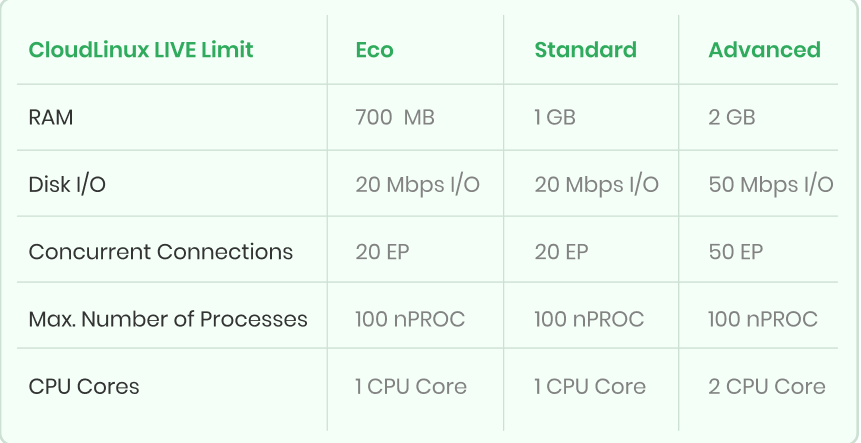
\includegraphics[width=0.7\linewidth]{7_2}
	\caption{using hardware list}
	\label{fig:72}
	\end{figure}
	\begin{figure}[h]
	\centering
	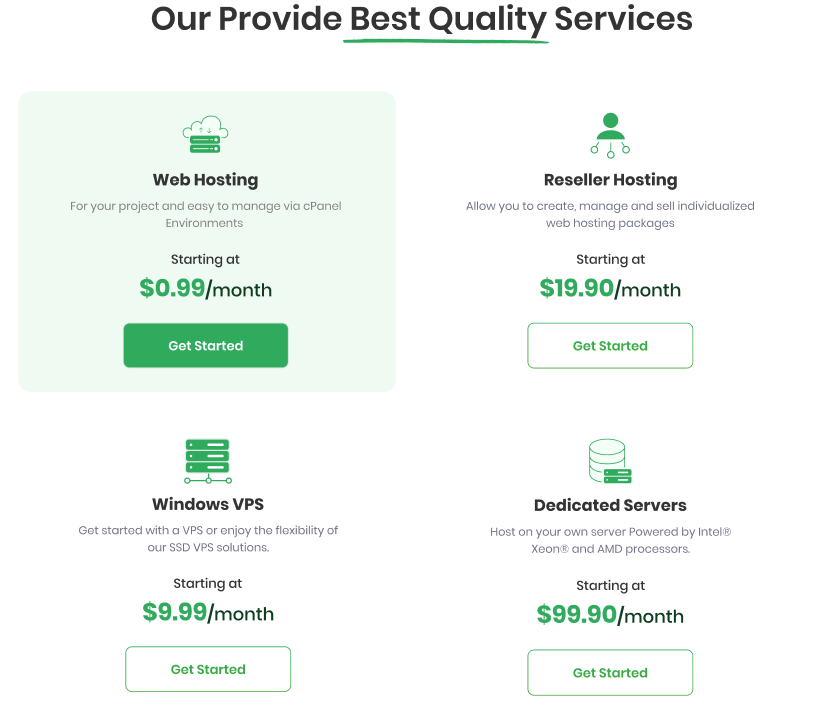
\includegraphics[width=0.8\linewidth]{8_4}
	\caption{NEtaCode services}
	\label{fig:84}
	\end{figure}

	\subitem \textbf{personnel cost:\\}It is the money send on the people involve in the development the project .These expenditures include salaries,other benifit such as health ,conveyance allowance etc.In netacode
	each personnel cost is 50000 per month and forevery project extra working per hours they pay extra 5000.
	\subitem \textbf{Time cost:} 
	If a project need to made by personnel more time ,give them more money.
	\newpage
\begin{figure}[h]
	\centering
	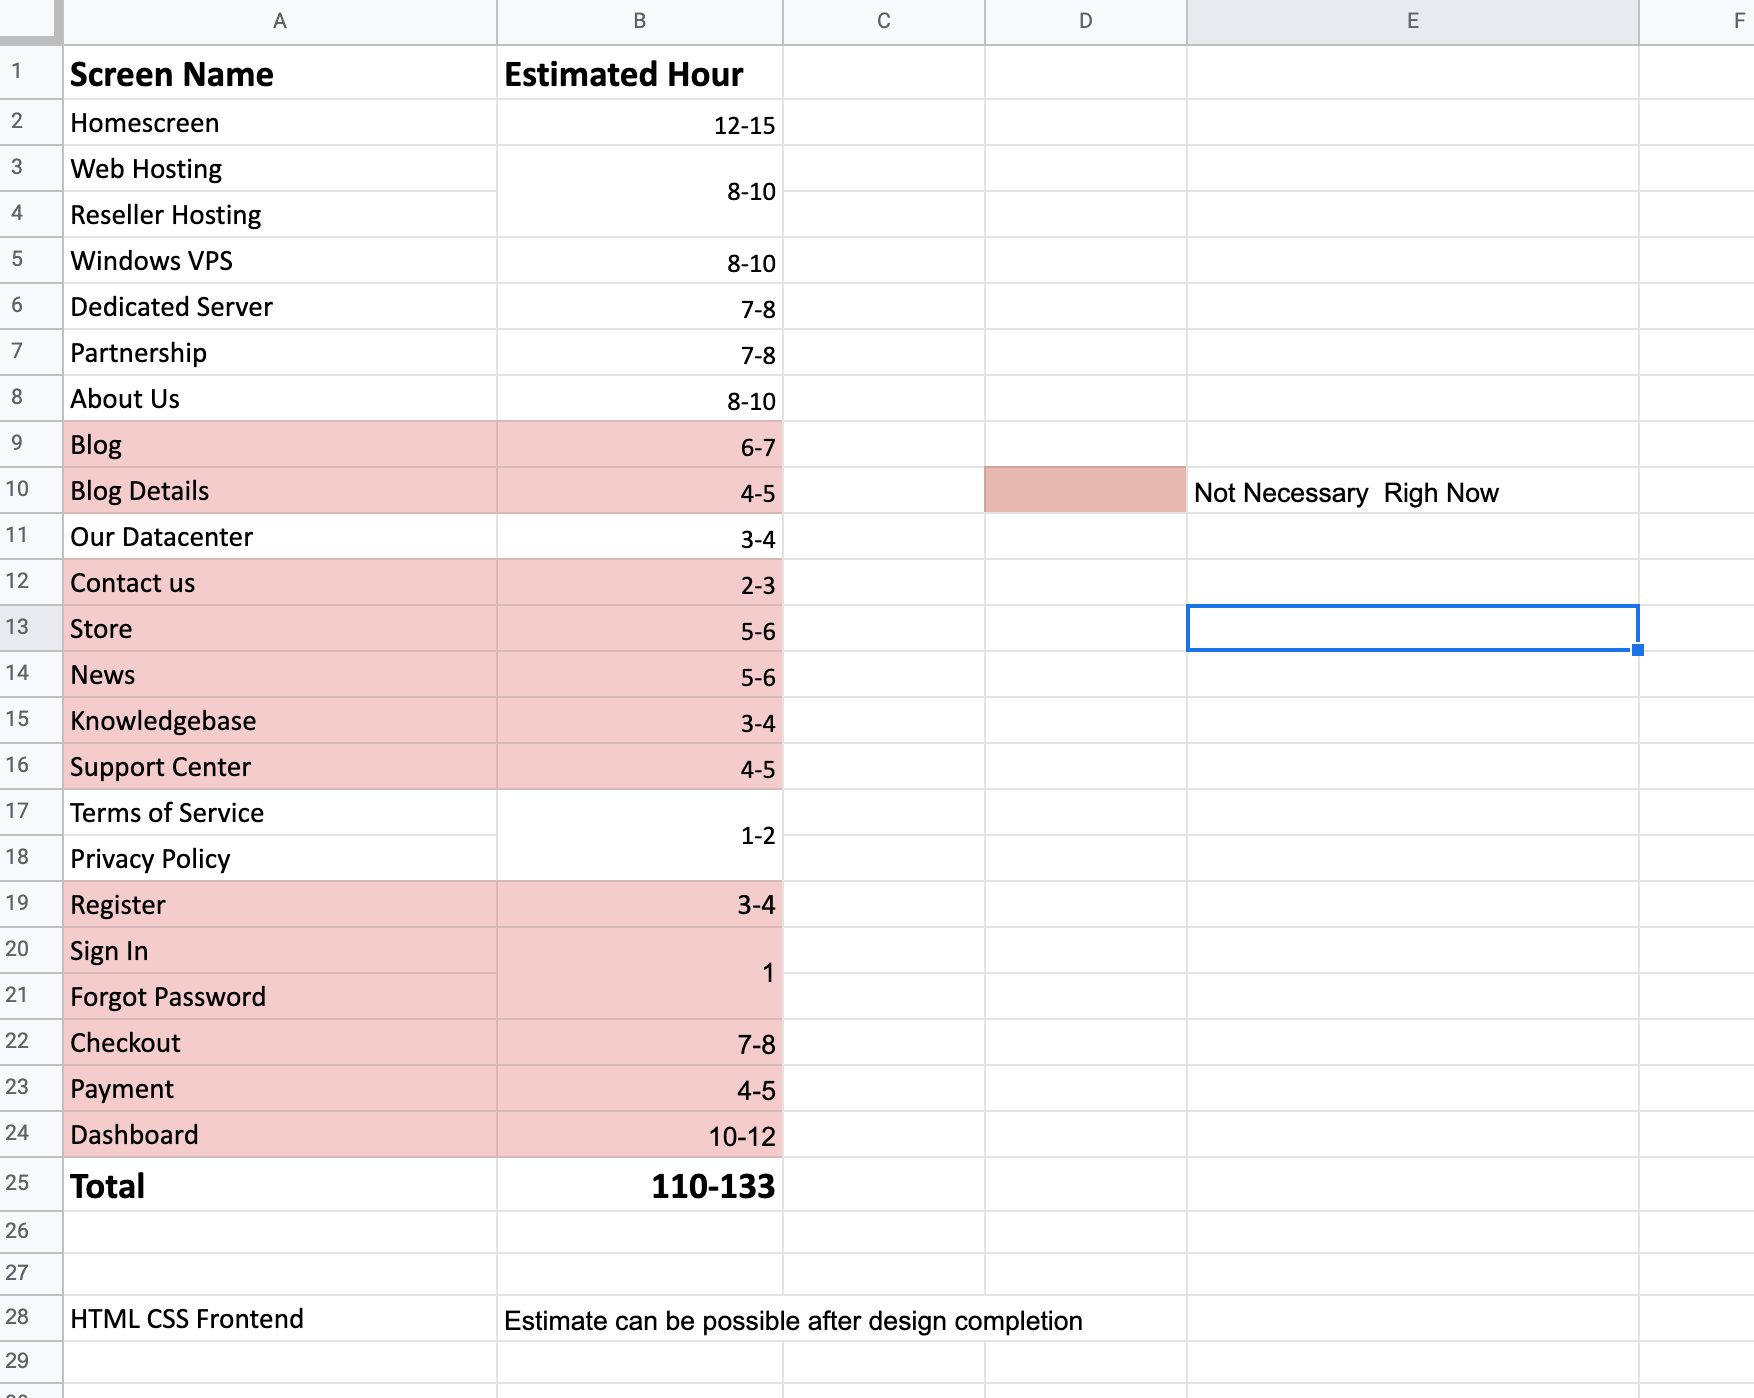
\includegraphics[width=1\linewidth]{8_1}
	\caption{Time requirement for a website ECNHOST made by NetaCode }
	\label{fig:81}
\end{figure}
\subsection{Cost analysis for a existing project}
Successfully run a project by Netacode cost analysis\\
Total Investment by clint is 3,550,000tk
\begin{center}
	 Ten member work in this project for 15 days.\\
 personnel cost =(10*50,000)+(5000*3*10)=6,50,000tk\\
 hardware/software cost=5,00000tk\\
 equipment cost=20,00000tk\\
 Others=4,00000\\
\end{center}
 \begin{center}
 	total=650000+500000+2000000+400000\\
 	      =3550000tk\\
 \end{center}

	\section{Benefit}
	The biggest advantage of Netacode audience is that -
	\begin{itemize}
		\item	clint can start with their services without any technical
		knowledge , as we will provide full support for them.
		\item Very Economical ( We can beat any of our competitors) with ensuring quality service
		\item Multi-Carrier Route Optimized Network
		\item Proactive monitoring and resolution
		\item Exceptional performance and reliability
		\item Best customer retention rate
		\item 24 hours Live Support by responsible and reliable Staff.
	\end{itemize} 
\subsection{Benefit analysis for a existing project}
After running the project average every month in first One year  earn by clint 150,000.\\
so,No.of month  need for net benifit\begin{center}
	n=3,550,000/200,000=~18 month=~1.8 year \\
	and every month server cost pay  by clint is 10,000tk
	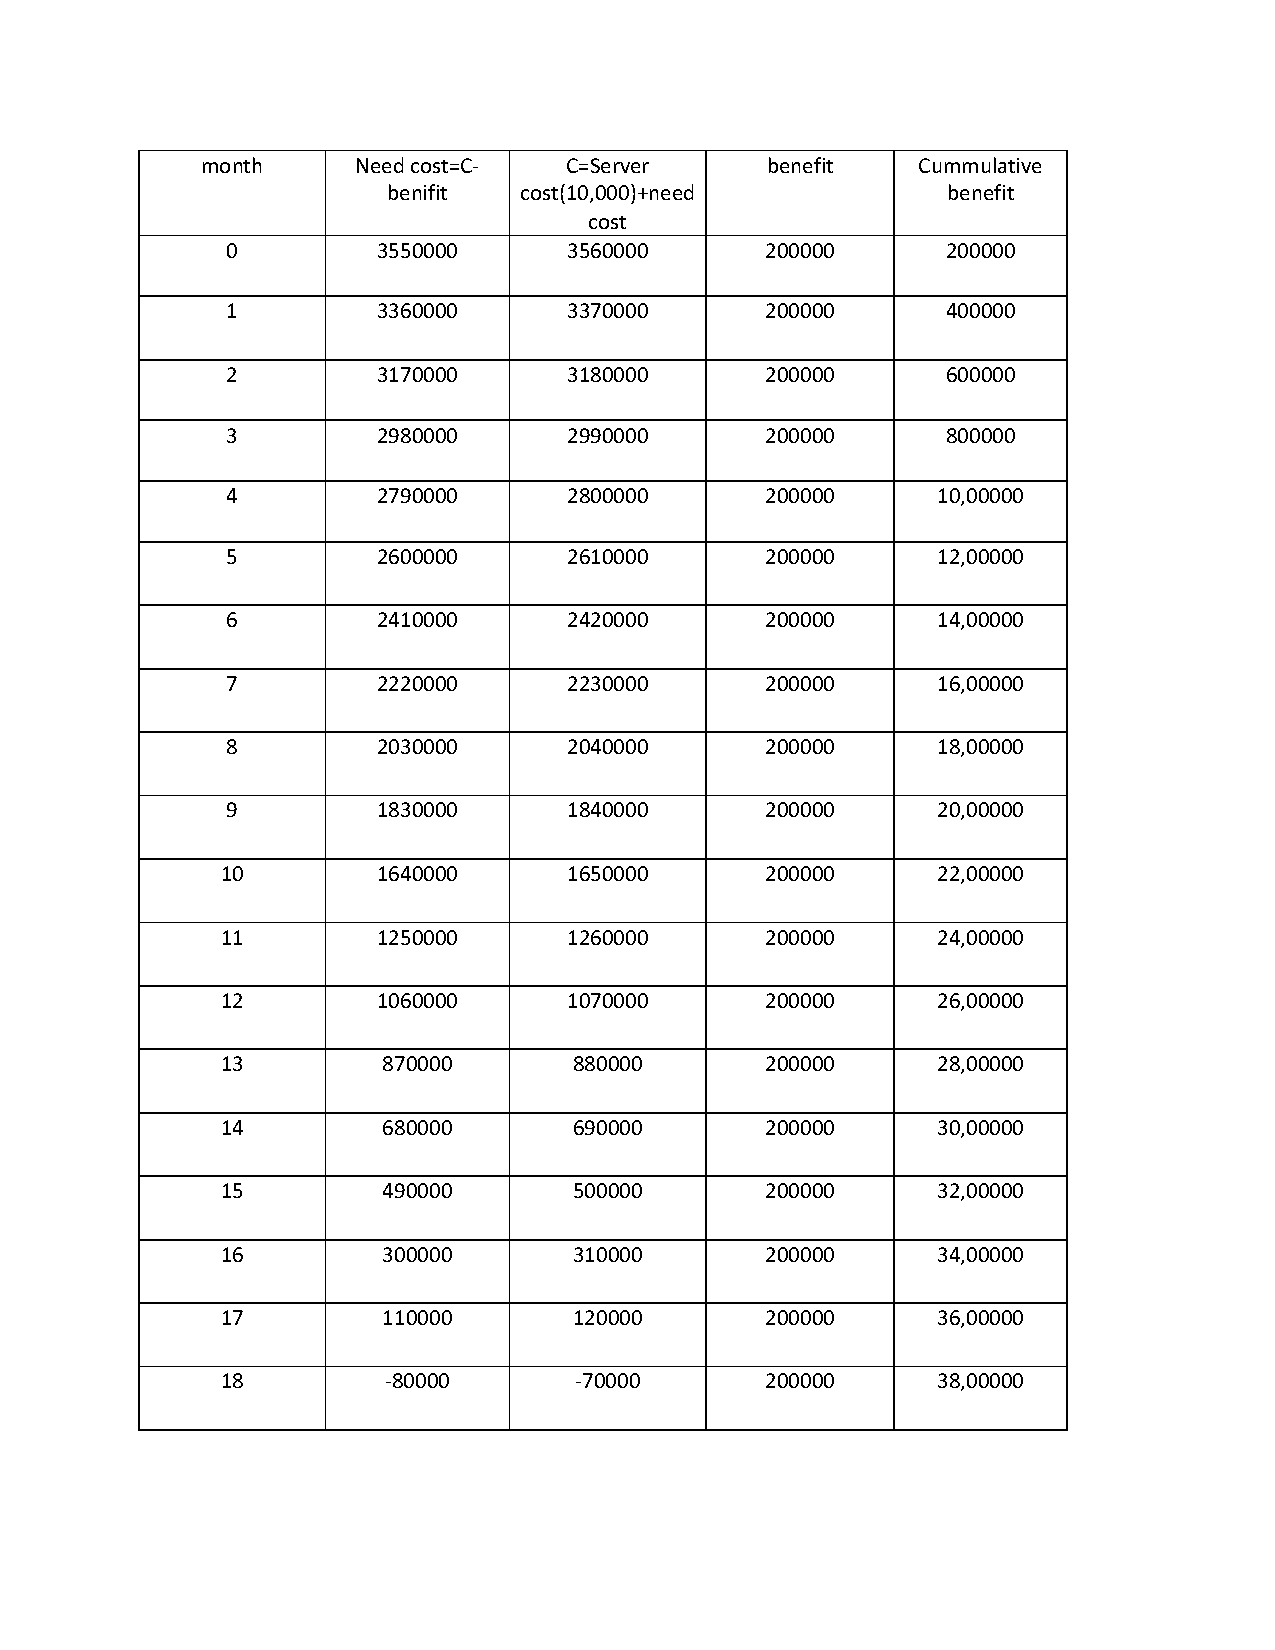
\includepdf[pages={1}] {cost.pdf}
\end{center} 
So after 18 month running this project the clint get 20,0000tk profit every month
\paragraph{Summary}
Cost benefit and data analysis is most Important think for every system.we can find the existing system is benifited or not after analysis cost and benefit analysis.Clint can decide the want run the system after seeing the cost analysis.
	
	\end{document}